\newpage
\subsection{Layouts} \index{Layouts}
Von den in Kapitel \refTC{sec:Activities} beschriebenen Activities besitzen \textit{CardActivity} und \textit{CardListActivity} ein dazugeh�riges Layout.

Das Layout von CardListActivity besteht neben den von Android vorgegebenen Teilen aus drei Parts. Zum ersten ist dies eine Listview, die es dem Programmier erlaubt, eine scrollbare Liste mit diversen Items zu erstellen. Die Aufgabe dieser Listview ist es, s�mtliche gespeicherten Garantiescheine darzustellen. 
Darunter folgt eine Zeile mit einer Checkbox, die f�r die Filterung der angezeigten Eintr�ge verantwortlich ist. 
Der unterste Teil wird von zwei Buttons belegt. �ber diese wird die App gesteuert.

%\begin{figure}[h!]
%\centering
%\begin{subfigure}{.4\textwidth}
%	\label{fig:CardListActivity_layout}
%	\centering
%	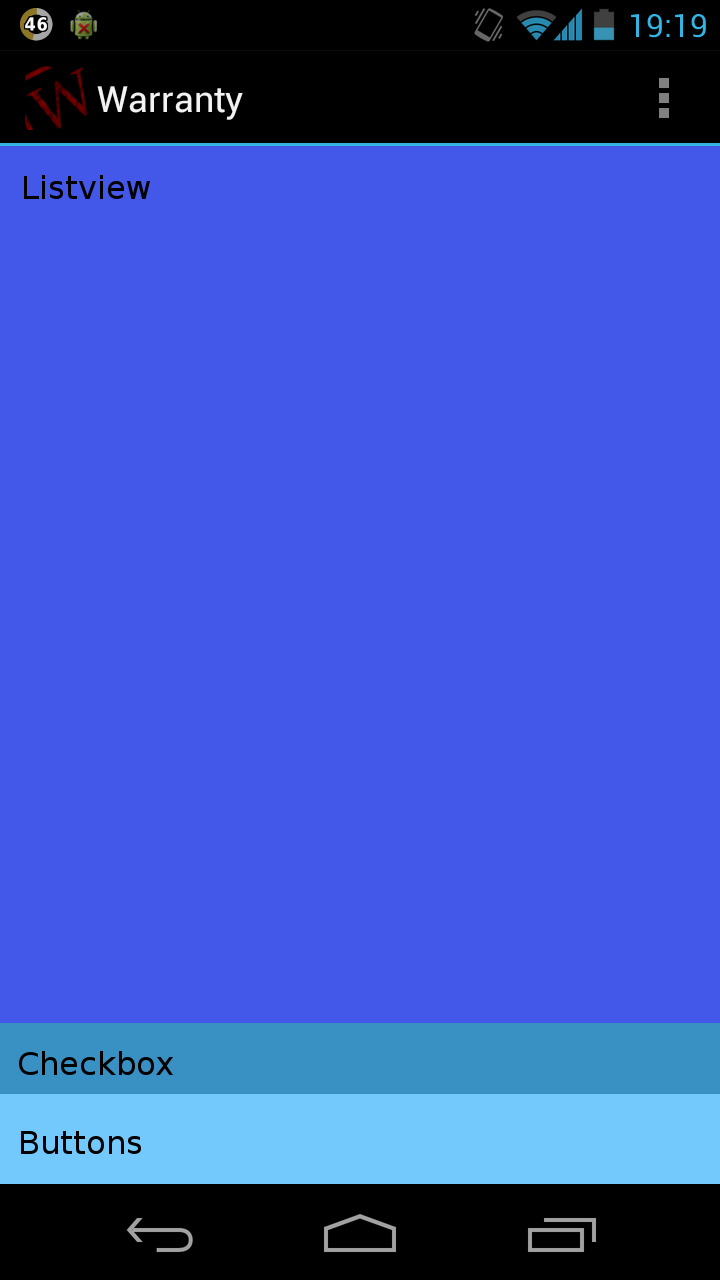
\includegraphics[width=0.8\linewidth]{CardListActivity_Layout.png} 
%	\caption{Aufbau Layout}
%\end{subfigure}
%\begin{subfigure}{.4\textwidth}
%	\label{fig:CardListActivity_layout}
%	\centering
%	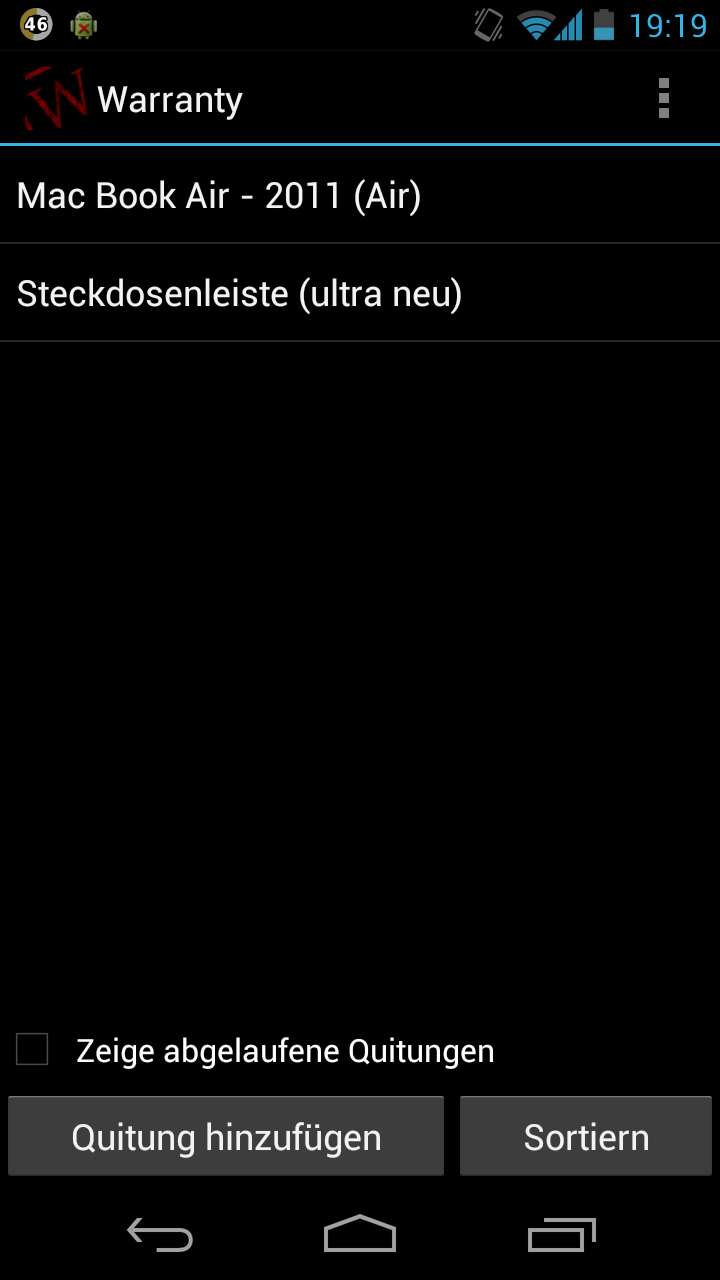
\includegraphics[width=0.8\linewidth]{Card_List_Activity_1.png} 
%	\caption{Umsetzung Layout}
%\end{subfigure}
%\caption{Layout CardListActivity}
%\end{figure}

\begin{figure}[h!]
\centering
\label{fig:CardListActivity_layout}
\begin{subfigure}{.3\textwidth}
	\centering
	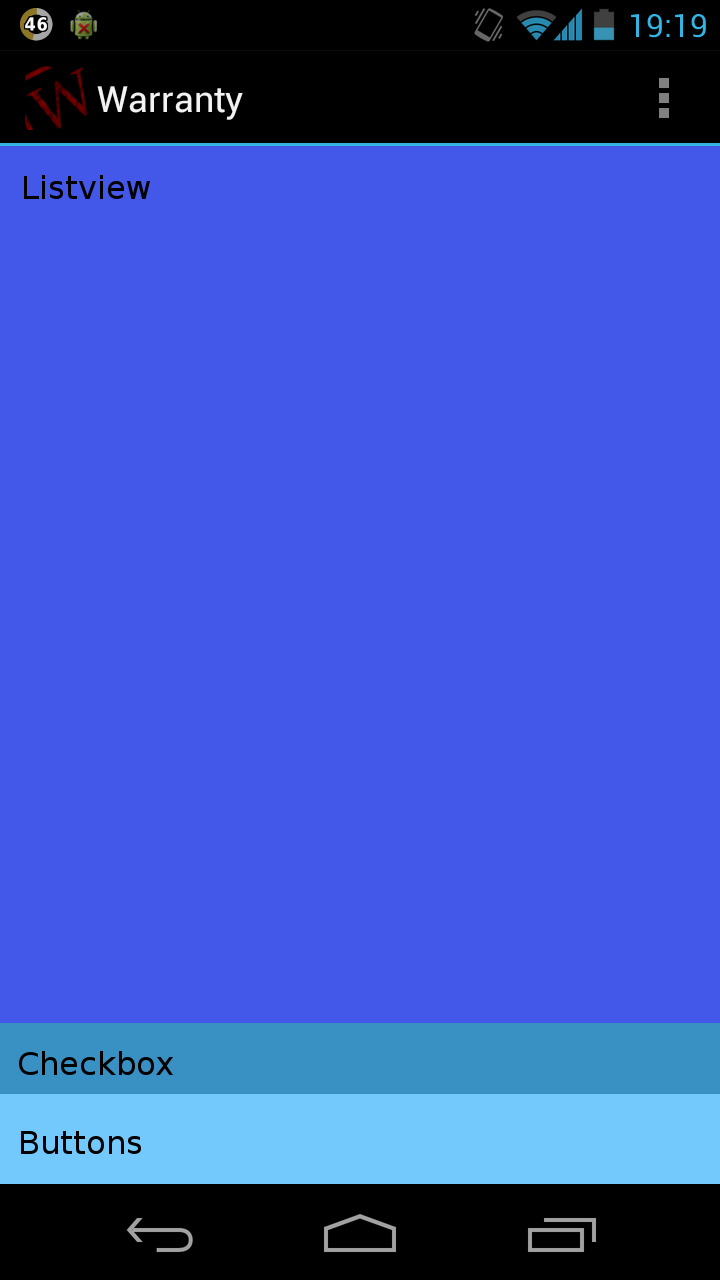
\includegraphics[width=0.8\linewidth]{CardListActivity_Layout.png} 
	\caption{Aufbau Layout}
\end{subfigure}
\begin{subfigure}{.3\textwidth}
	\centering
	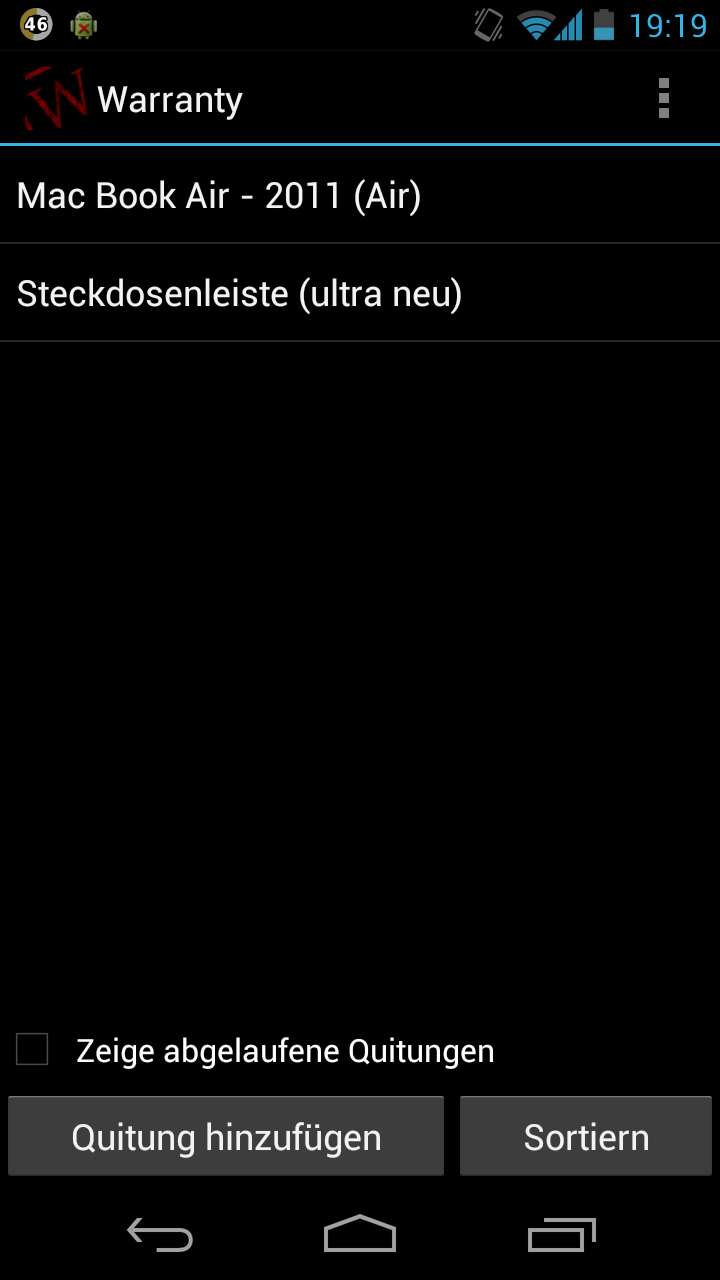
\includegraphics[width=0.8\linewidth]{Card_List_Activity_1.png} 
	\caption{Umsetzung Layout}
\end{subfigure}
\begin{subfigure}{.3\textwidth}
	\centering
	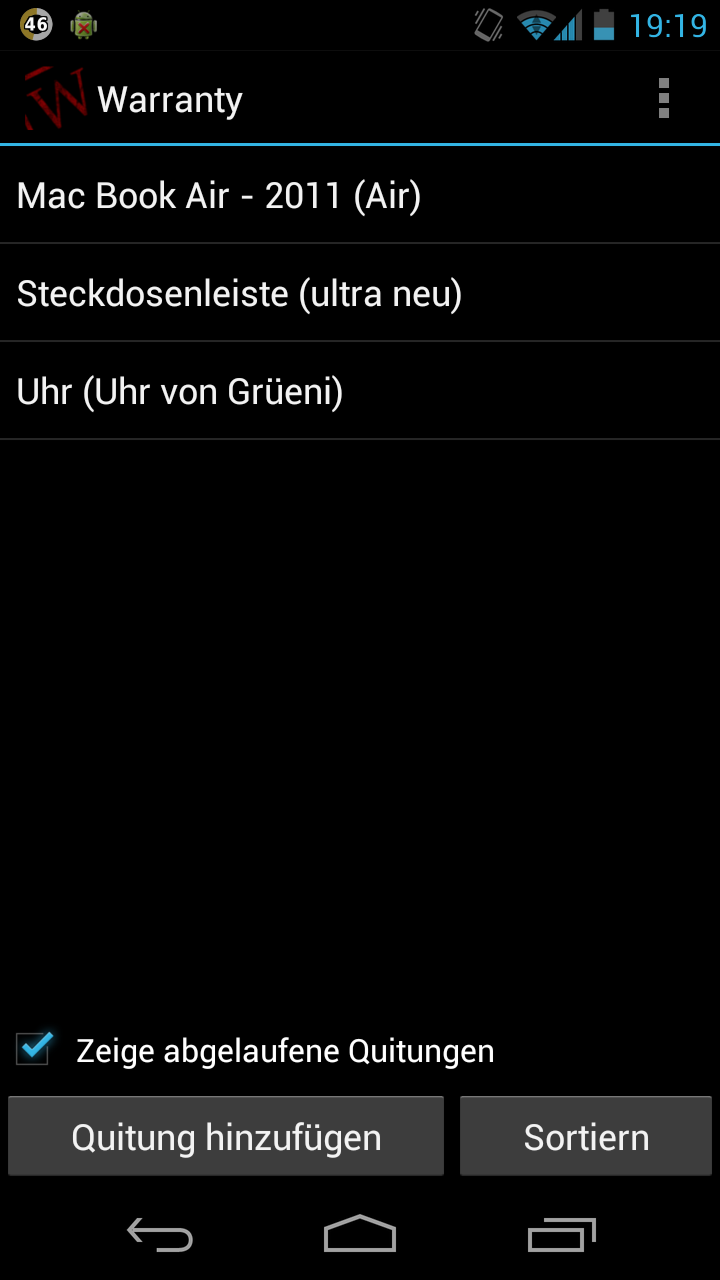
\includegraphics[width=0.8\linewidth]{Card_List_Activity_2.png} 
	\caption{Umsetzung Layout}
\end{subfigure}
\caption{Layout CardListActivity}
\end{figure}

\newpage
Das zweite Layout, das CardActivity Layout besteht aus mehreren Komponenten. Die wichtigste Rolle spielen hier die verschiedenen EditText- Felder, die zur Eingabe von Daten ben�tigt werden. Daneben existieren diverse Buttons, beispielsweise um das Erstellungs- bzw. das Auslaufdatum eines Garantiescheines zu erfassen. Im untersten Drittel des Bildschirms ist eine ImageView zum darstellen von Bildern untergebracht.

\begin{figure}[h!]
\centering
\label{fig:CardActivity_layout}
\begin{subfigure}{.4\textwidth}
	\centering
	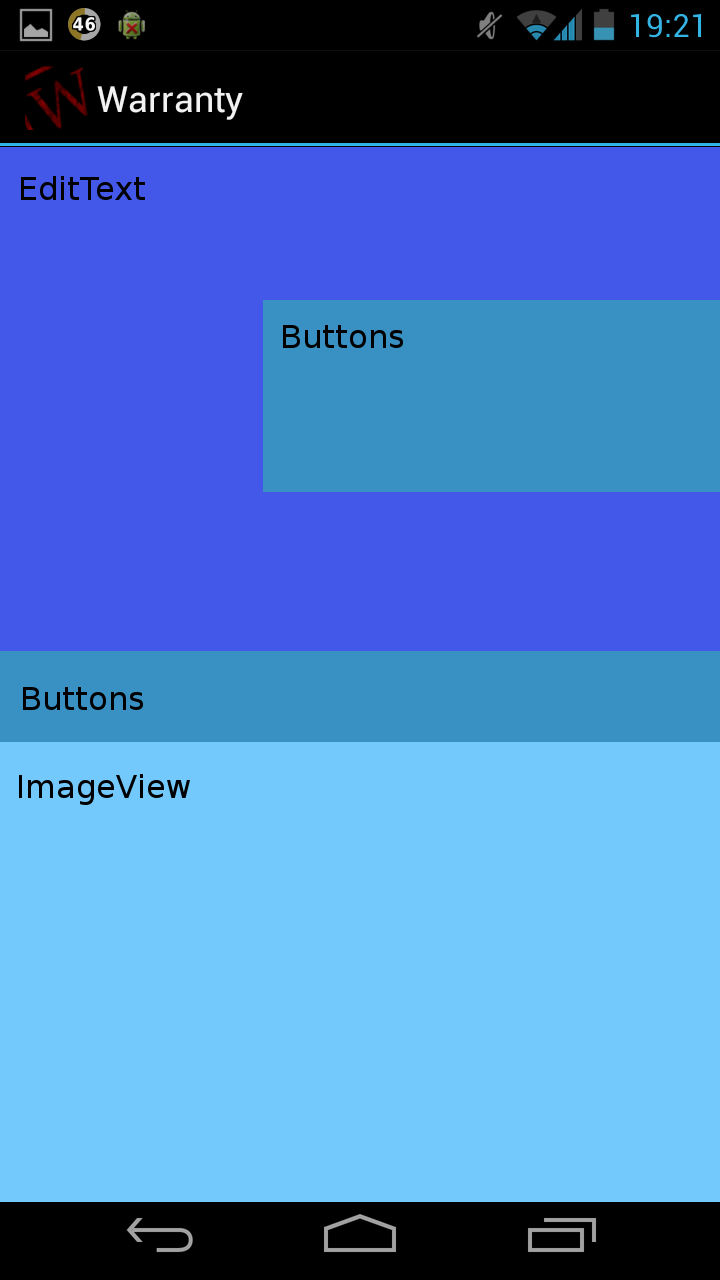
\includegraphics[width=0.8\linewidth]{CardActivity_Layout.png} 
	\caption{Aufbau Layout}
\end{subfigure}
\begin{subfigure}{.4\textwidth}
	\centering
	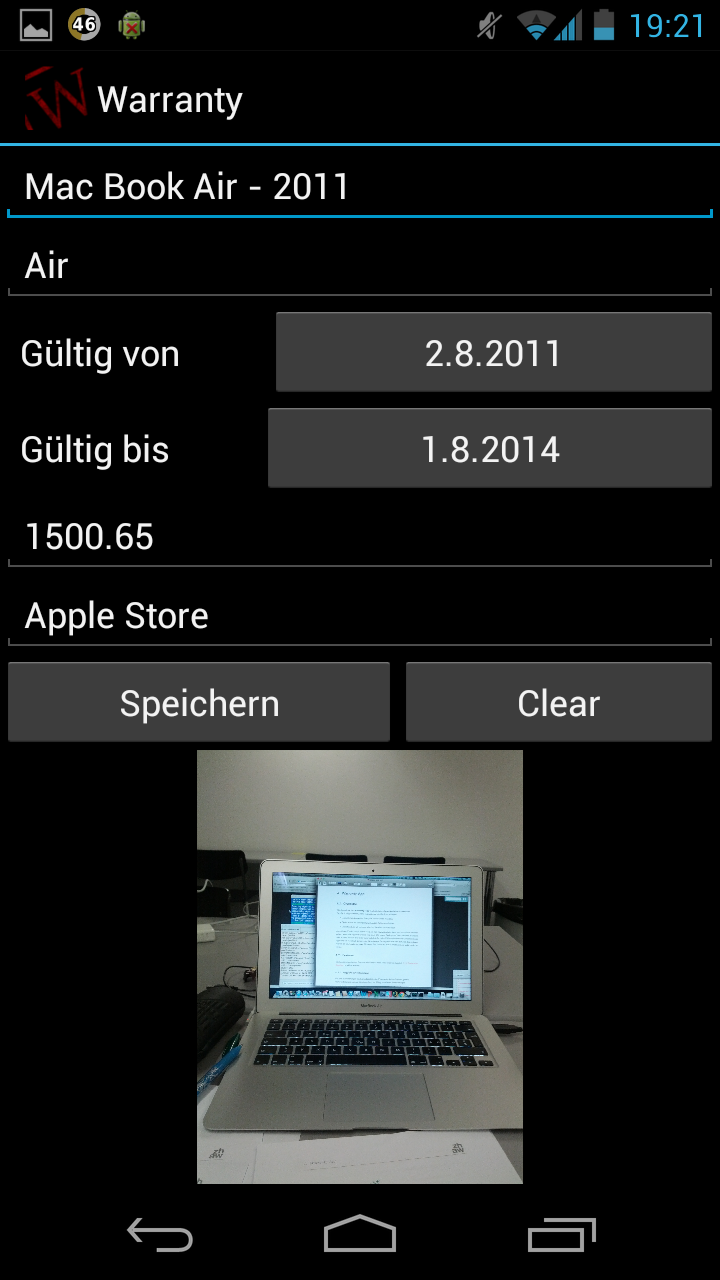
\includegraphics[width=0.8\linewidth]{Card_Activity.png} 
	\caption{Umsetzung Layout}
\end{subfigure}
\caption{Layout CardActivity}
\end{figure}

